\section{Kinematics for the Geomagic touch}

As shown on \figref{fig:phantom_omni}, the Phantom omni has 6 joints.
The coordinate frame for these joints can be derived as shown on \figref{fig:Frame_phantom}. 
The 6 frames on the DH scheme correspond to the links on the Geomagic touch and define their orientation and position.



\begin{minipage}[H]{.65\textwidth}
\centering
\begin{figure}[H]
\centering
\vspace{0pt}
%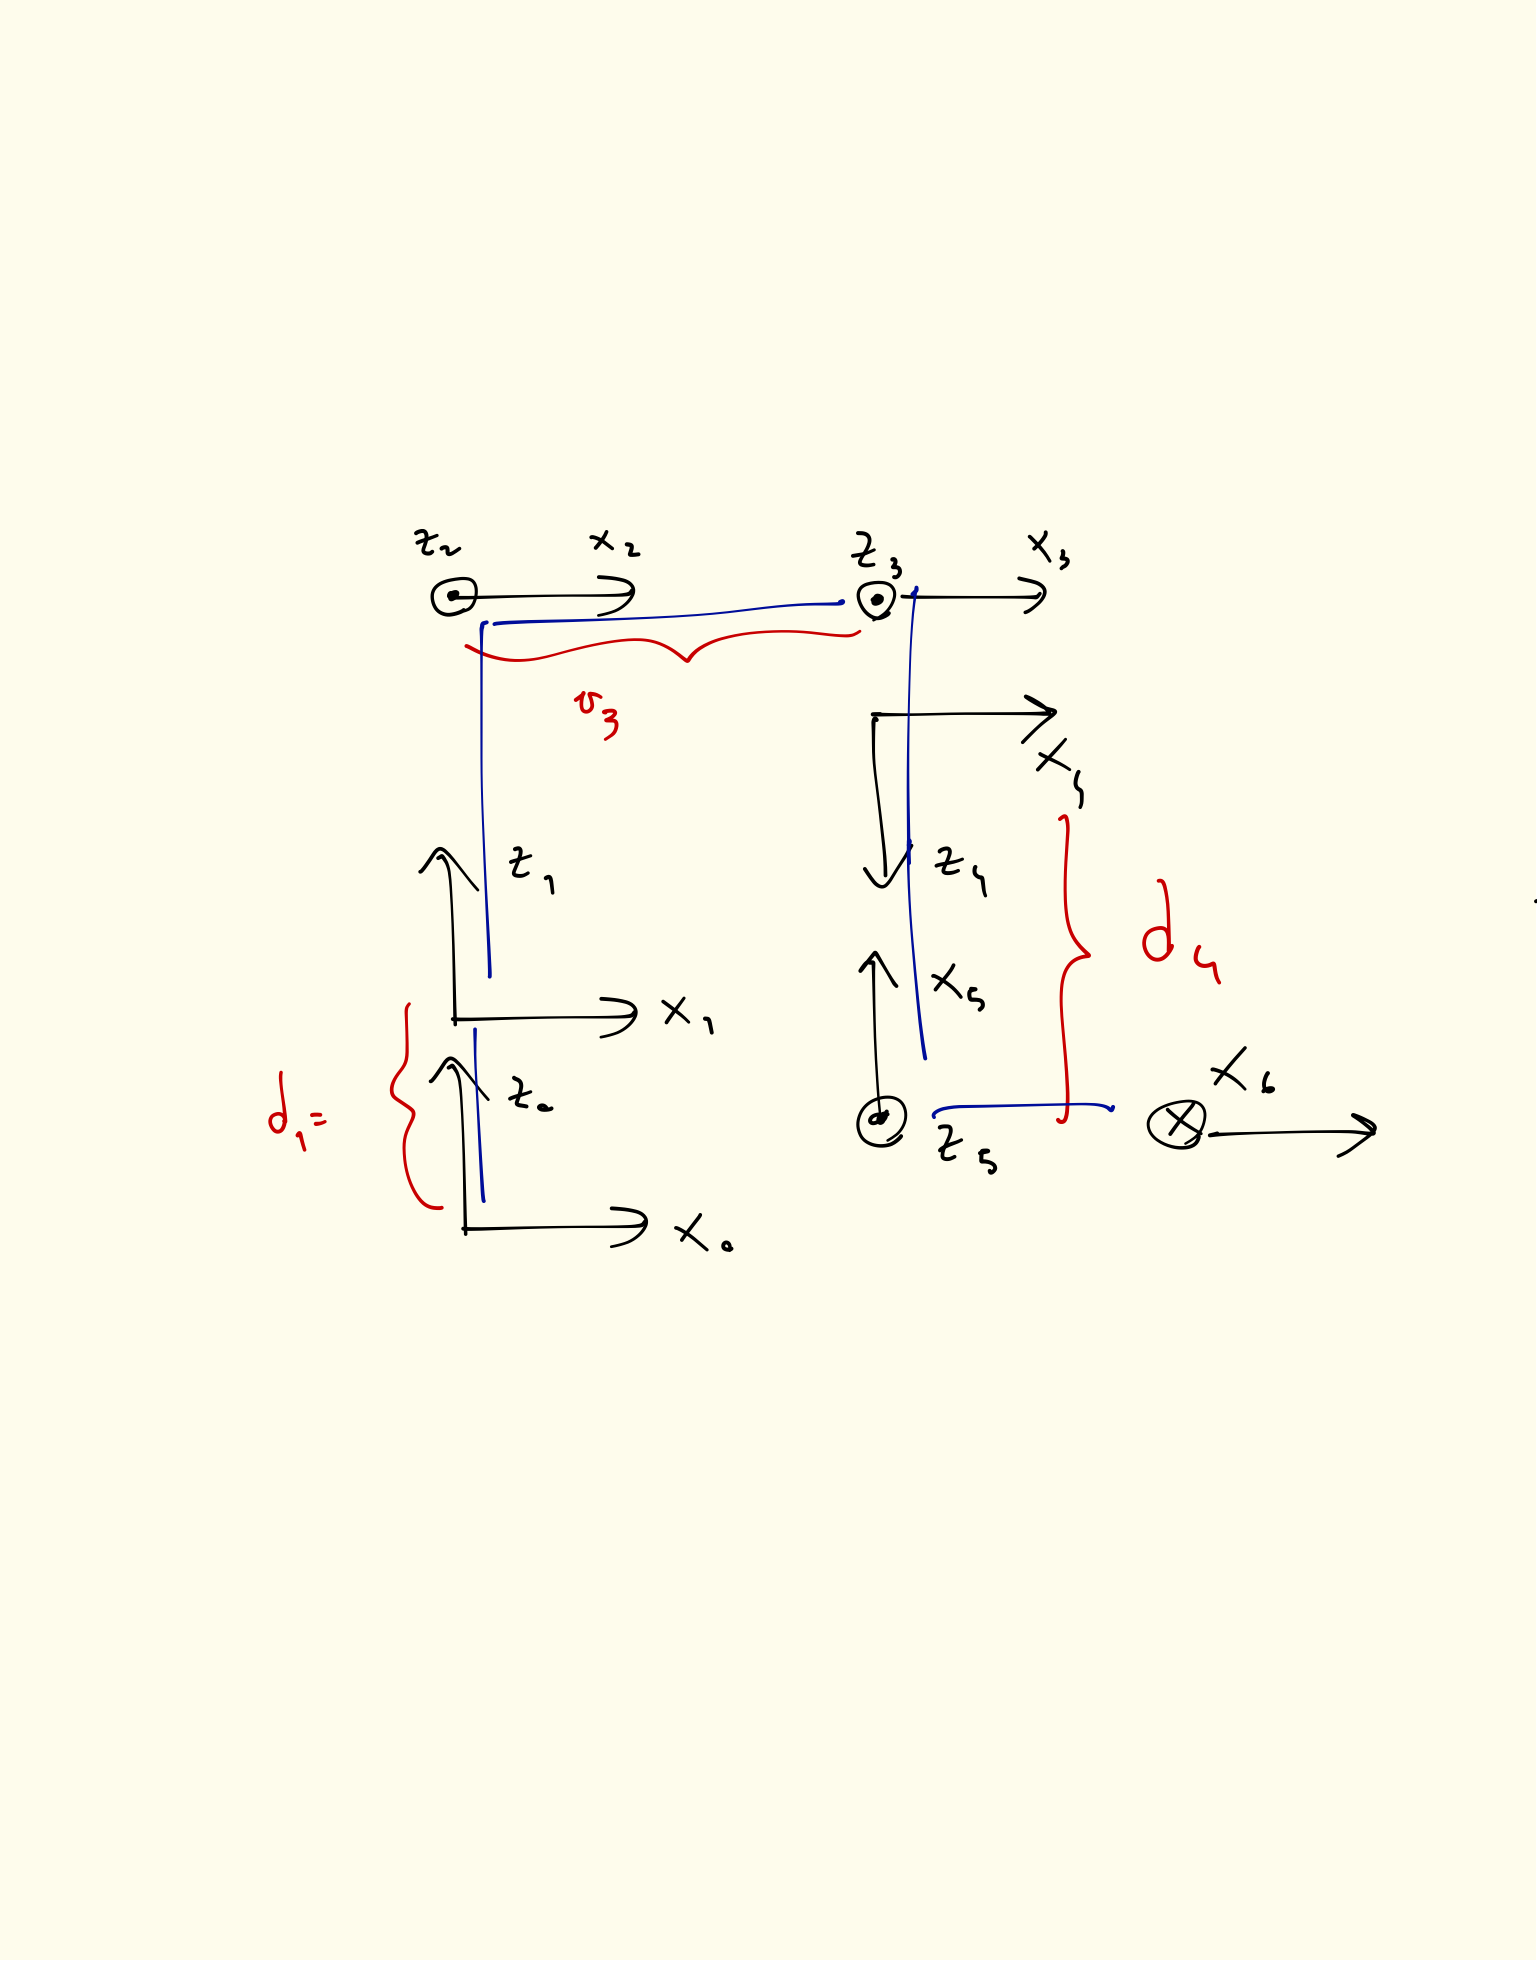
\includegraphics[width=\textwidth]{Geomagic_dh.png}

\begin{scaletikzpicturetowidth}{0.85\textwidth}
\begin{tikzpicture}[scale=\tikzscale]

\node at (-0.25,-0.25) {$O_0$};
\draw [<->,ultra thick] (2,0) -- (0,0) -- (0,2);
\node at (2.5,0) {$x_0$};
\node at (-0.5,2) {$z_0$};

\draw [blue,thick, decorate,decoration={brace,amplitude=10pt},xshift=-4pt,yshift=0pt]
(-0.55,0) -- (-0.55,2.5) node [black,midway,xshift=-0.6cm] 
{\footnotesize $d_1$};

\draw [<->,ultra thick] (2,2.5) -- (0,2.5) -- (0,4.5);
\node at (2.5,2.5) {$x_1$};
\node at (-0.5,4.5) {$z_1$};

\draw [->,ultra thick] (0,6) -- (2,6);
\draw [fill=red] (0,6) circle [radius=0.1];
\draw [thick] (0,6) circle [radius=0.2];
\node at (0,6.6) {$z_2$};
\node at (2,6.6) {$x_2$};

\draw [blue,thick,decorate,decoration={brace,amplitude=10pt,mirror,raise=4pt},yshift=0pt]
(0,5.8) -- (5,5.8) node [black,midway,xshift=0cm,yshift=-0.7cm] {\footnotesize
$a_3$};

\draw [->,ultra thick] (5,6) -- (7,6);
\draw [fill=red] (5,6) circle [radius=0.1];
\draw [thick] (5,6) circle [radius=0.2];
\node at (5,6.6) {$z_3$};
\node at (7,6.6) {$x_3$};

\draw [<->,ultra thick] (5,2.5) -- (5,4.5) -- (7,4.5);
\node at (7,5) {$x_4$};
\node at (4.5,2.5) {$z_4$};

\draw [->,ultra thick] (5,0) -- (5,2);
\draw [fill=red] (5,0) circle [radius=0.1];
\draw [thick] (5,0) circle [radius=0.2];
\node at (4.5,0) {$z_5$};
\node at (4.5,2) {$x_5$};

\draw [blue,thick, decorate,decoration={brace,amplitude=10pt},xshift=-4pt,yshift=0pt]
(4.3,0) -- (4.3,4.5) node [black,midway,xshift=-0.6cm] 
{\footnotesize $d_4$};

\draw [->,ultra thick] (6.6,0) -- (8.5,0);
\draw [thick] (6.5,0) circle [radius=0.2];
\node [red, ultra thick] at (6.5,0) {x};
\node at (6.5,0.5) {$x_6$};

\draw [fill=red] (-1,-1) circle [radius=0.1];
\draw [thick] (-1,-1) circle [radius=0.2];
\node at (2.6,-0.95) {z axis outwards direction.};

\draw [thick] (-1,-1.5) circle [radius=0.2];
\node [red, ultra thick] at (-1,-1.5) {x};
\node at (2.5,-1.5) {z axis inwards direction.};

\end{tikzpicture}
\end{scaletikzpicturetowidth}

\caption{Coordinate frame for the\newline Geomagic Touch.}
\label{fig:Frame_phantom}
\end{figure}
\end{minipage}%\hfill
\begin{minipage}[H]{.35\textwidth}
\begin{table}[H]
\centering
\vspace{95pt}
\begin{tabular}{|l|l|l|l|l|}
\hline
 $j_i$ 	  & $a_i$    & $d_i$ & $\alpha_i$ 		 & $\theta_i$ 			 \\ \hline
 1  	  &  $0$     & $d_1$ & $0$	 & $q_1$ 			     \\ \hline
 2  	  &  $0$   & $0$ 	 & $\frac{\pi}{2}$ 		 		 & $q_2 + \theta_1$ 	 \\ \hline
 3  	  &  $a_3$	 & $0$ & $0$ 		 		 & $q_3$ 					 \\ \hline
 4  	  &  $0$	 & $d_4$ & $\frac{\pi}{2}$ 	 & $q_4$ 			 \\ \hline
 5  	  &  $0$	 & $0$ & $-\frac{\pi}{2}$ 		 		 & $-\frac{\pi}{2} + q_5$ 	 				 \\ \hline
 6  	  &  $0$	 & $0$ & $-\frac{\pi}{2}$ 		 & $\frac{\pi}{2}+q_6$ 				 \\ \hline
\end{tabular}
\hspace{2cm}\caption{The DH notations for the\newline Geomagic Touch}
\label{tab:kin_geo}
\end{table}
\end{minipage}

\todo{new figure}








% \begin{figure}[H]
% 	\centering
% 	\begin{subfigure}{.49\textwidth}
% 		\centering
% 		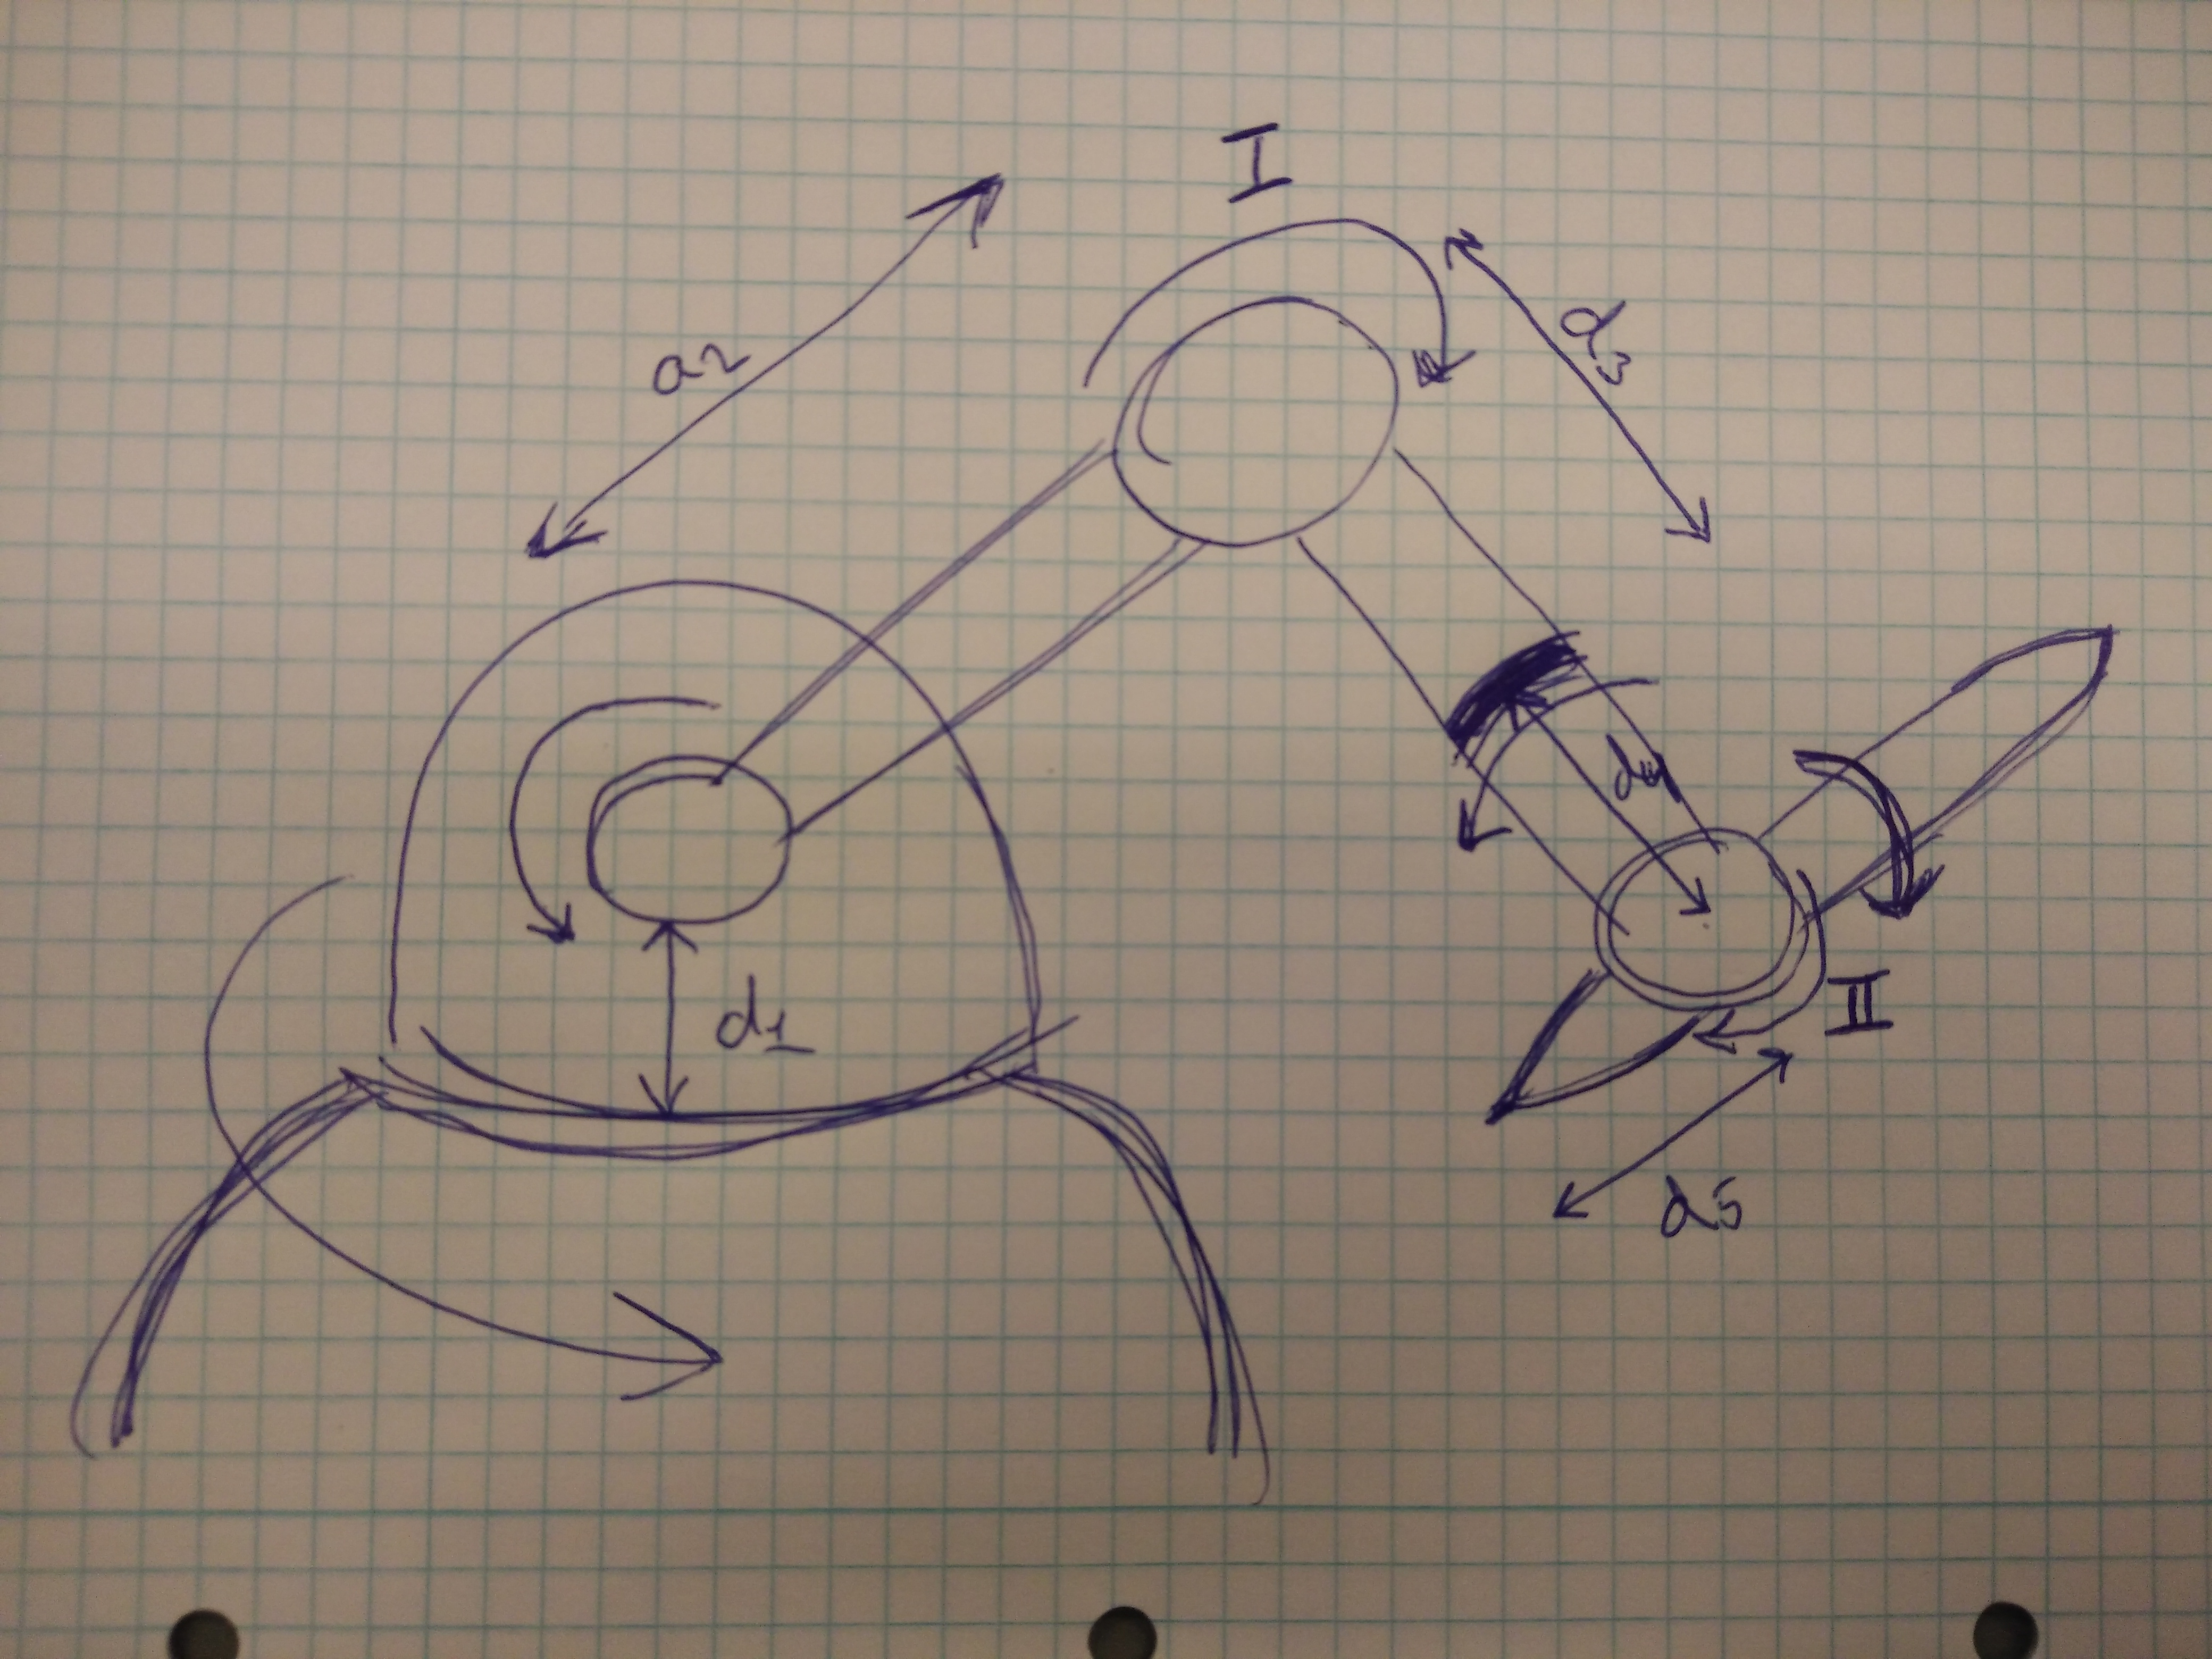
\includegraphics[width=\linewidth]{Fast_draw_Kino.jpg}
% 		\caption{Geomagic touch with all rotational joints and their \gls{DH} parameters.}
% 		\label{fig:1}
% 	\end{subfigure}
% 	\begin{subfigure}{.49\textwidth}
% 		\centering
% 		\includegraphics[width=\linewidth]{Fast_draw_kino2.jpg}
% 		\caption{Frame coordinate system for the Geomagic touch to the deviation of the kinematics.}
% 		\label{fig:Endo_plates}
% 	\end{subfigure}
% \caption{Shows joints positions, the different \gls{DH} parameters and the coordinate frame for each joint. The base frame is difined as $O_{0}$.}
% \label{fig:2}
% \end{figure}


% \begin{table}[H]
% \centering
% \begin{tabular}{|l|l|l|l|l|}
% \hline
%  $j_i$ 	  & $a_i$    & $d_i$ & $\alpha_i$ 		 & $\theta_i$ 			 \\ \hline
%  1  	  &  $0$     & $d_1$ & $\frac{\pi}{2}$	 & $q_1$ 			     \\ \hline
%  2  	  &  $a_2$   & $0$ 	 & $0$ 		 		 & $q_2 + \theta_1$ 	 \\ \hline
%  \rom{1}  &  $0$	 & $0$ 	 & $\frac{\pi}{2}$ 	 & $\frac{\pi}{2} + q_3$ \\ \hline
%  3  	  &  $0$	 & $d_3$ & $0$ 		 		 & $0$ 					 \\ \hline
%  4  	  &  $0$	 & $d_4$ & $\frac{\pi}{2}$ 	 & $\pi + q_4$ 			 \\ \hline
%  \rom{2}  &  $0$	 & $0$ 	 & $\frac{\pi}{2}$   & $\pi +q_5$ 			 \\ \hline
%  5  	  &  $0$	 & $d_5$ & $0$ 		 		 & $0$ 	 				 \\ \hline
%  %6  	  &  $0$	 & $d_6$ & $\theta$ 		 & $q_6$ 				 \\ \hline
% \end{tabular}
% \caption{Tabular which contain the kinematics for the Geomagic touch described in \secref{sec:geo_magic}.The Roman numbers defines the fictional joints}
% \label{tab:kin_geo}
% \end{table}